\documentclass[handout]{beamer}
\usetheme{Marburg}
\useoutertheme{infolines}
\newcommand{\answers}{1}

\usepackage{amsmath}
\usepackage{caption}
\usepackage{color}
\usepackage{enumerate}
\usepackage{listings}
\usepackage{hyperref}
\usepackage{mathrsfs}
\usepackage{natbib}
\usepackage{url}

\providecommand{\all}{\ \forall \ }
\providecommand{\bs}{\backslash}
\providecommand{\e}{\varepsilon}
\providecommand{\E}{\ \exists \ }
\providecommand{\lm}[2]{\lim_{#1 \rightarrow #2}}
\providecommand{\m}[1]{\mathbb{#1}}
\providecommand{\nv}{{}^{-1}}
\providecommand{\ov}[1]{\overline{#1}}
\providecommand{\p}{\newpage}
\providecommand{\q}{$\quad$ \newline}
\providecommand{\rt}{\rightarrow}
\providecommand{\Rt}{\Rightarrow}
\providecommand{\vc}[1]{\boldsymbol{#1}}
\providecommand{\wh}[1]{\widehat{#1}}

\hypersetup{colorlinks,linkcolor=,urlcolor=blue}
\numberwithin{equation}{section}

\definecolor{dkgreen}{rgb}{0,0.6,0}
\definecolor{gray}{rgb}{0.5,0.5,0.5}
\definecolor{mauve}{rgb}{0.58,0,0.82}

\lstset{ 
  language=C,                % the language of the code
  basicstyle= \footnotesize,           % the size of the fonts that are used for the code
  numbers=left,
  numberfirstline=true,
  numbersep=5pt,                  % how far the line-numbers are from the code
  backgroundcolor=\color{white},      % choose the background color. You must add \usepackage{color}
  showspaces=false,               % show spaces adding particular underscores
  showstringspaces=false,         % underline spaces within strings
  showtabs=false,                 % show tabs within strings adding particular underscores
  frame=lrb,                   % adds a frame around the code
  rulecolor=\color{black},        % if not set, the frame-color may be changed on line-breaks within not-black text 
  tabsize=2,                      % sets default tabsize to 2 spaces
  captionpos=t,                   % sets the caption-position 
  breaklines=true,                % sets automatic line breaking
  breakatwhitespace=false,        % sets if automatic breaks should only happen at whitespace
  %title=\lstname,                   % show the filename of files included with \lstinputlisting;
  keywordstyle=\color{blue},          % keyword style
  commentstyle=\color{gray},       % comment style
  stringstyle=\color{dkgreen},         % string literal style
  escapeinside={\%*}{*)},            % if you want to add LaTeX within your code
  morekeywords={*, ...},               % if you want to add more keywords to the set
  xleftmargin=0.053in, % left horizontal offset of caption box
  xrightmargin=-.03in % right horizontal offset of caption box
}

%\DeclareCaptionFont{white}{\color{white}}
%\DeclareCaptionFormat{listing}{\parbox{\textwidth}{\colorbox{gray}{\parbox{\textwidth}{#1#2#3}}\vskip-0.05in}}
%\captionsetup[lstlisting]{format = listing, labelfont = white, textfont = white}
%For caption-free listings, comment out the 3 lines above and uncomment the 2 lines below.
 \captionsetup{labelformat = empty, labelsep = none}
 \lstset{frame = single}

\title{The PyCUDA module}
\author{Will Landau}
\date{December 2, 2013}
\institute{Iowa State University}

\begin{document}

\begin{frame}
\titlepage
 \end{frame}
 
 \begin{frame}
\frametitle{Outline}
\tableofcontents
\end{frame}
 
 \AtBeginSection[]
{
   \begin{frame}
       \frametitle{Outline}
       \tableofcontents[currentsection]
   \end{frame}
}

\section{Getting started}

\begin{frame}[fragile]
\frametitle{\tt demo.py}
\begin{itemize}
\item Import and initialize PyCUDA:
\begin{lstlisting}[name=dp]
import pycuda.driver as cuda
import pycuda.autoinit
from pycuda.compiler import SourceModule
\end{lstlisting}
\pause \item Initial data: a 4 $\times$ 4 array of numbers:
\begin{lstlisting}[name=dp]
import numpy
a = numpy.random.randn(4,4)
\end{lstlisting}
\pause \item Many NVIDIA cards only support single precision:
\begin{lstlisting}[name=dp]
a = a.astype(numpy.float32)
\end{lstlisting}
\end{itemize}
\end{frame}

\begin{frame}[fragile]
\frametitle{\tt demo.py}
\begin{itemize}
\item Allocate device memory:
\begin{lstlisting}[name=dp]
a_gpu = cuda.mem_alloc(a.nbytes)
\end{lstlisting}
\pause \item Send data to the device: 
\begin{lstlisting}[name=dp]
cuda.memcpy_htod(a_gpu, a)
\end{lstlisting}
\pause \item Define a kernel to multiply each array entry by 2:
\begin{lstlisting}[name=dp]
mod = SourceModule("""
  __global__ void doublify(float *a)
  {
    int idx = threadIdx.x + threadIdx.y*4;
    a[idx] *= 2;
  }
  """)
\end{lstlisting}
\end{itemize}
\end{frame}

\begin{frame}[fragile]
\frametitle{\tt demo.py}
\begin{itemize}
\item Turn our CUDA C kernel into a callable Python function:
\begin{lstlisting}[name=dp]
func = mod.get_function("doublify")
\end{lstlisting}
\pause \item Call the kernel with:
\begin{itemize}
\item 1 grid
\item 1 block
\item 4 threads in the x direction
\item 4 threads in the y direction
\item 1 thread in the z direction
\end{itemize}
\pause \begin{lstlisting}[name=dp]
func(a_gpu, block=(4,4,1))
\end{lstlisting}
\end{itemize}
\end{frame}

\begin{frame}[fragile]
\frametitle{\tt demo.py}
\begin{itemize}
\item Make a NumPy array to store the results:
\begin{lstlisting}[name=dp]
a_doubled = numpy.empty_like(a)
\end{lstlisting}
\pause \item Copy the results to the host:
\begin{lstlisting}[name=dp]
cuda.memcpy_dtoh(a_doubled, a_gpu)
\end{lstlisting}
\pause \item Print arrays:
\begin{lstlisting}[name=dp]
print a_doubled
print a
\end{lstlisting}
\end{itemize}
\end{frame}

\begin{frame}[fragile]
\frametitle{Example output}

\lstset{basicstyle=\tiny}
\begin{lstlisting}
[landau@impact1 PyCUDA_sandbox]$ python demo.py
[[-1.29063177  0.82264316  0.02254304  2.0740006 ]
 [ 1.40431428  1.95245779 -1.84627843 -1.5800966 ]
 [-2.77298713  0.99803442  1.85154581  0.63633269]
 [ 0.55860651 -0.50091052 -1.465307    4.12601614]]
[[-0.64531589  0.41132158  0.01127152  1.0370003 ]
 [ 0.70215714  0.97622889 -0.92313921 -0.7900483 ]
 [-1.38649356  0.49901721  0.92577291  0.31816635]
 [ 0.27930325 -0.25045526 -0.7326535   2.06300807]]
\end{lstlisting}
\end{frame}

\begin{frame}
\frametitle{Simplifying memory transfer}
\begin{itemize}
\item There are three function argument handlers that take care of memory transfer for the user:
\begin{itemize}
\item {\tt pycuda.driver.In}
\item {\tt pycuda.driver.Out}
\item {\tt pycuda.driver.InOut}
\end{itemize}
\end{itemize}
\end{frame}

\lstset{basicstyle=\tiny}

\begin{frame}[fragile]
\frametitle{{\tt hello\_gpu.py}}
\begin{lstlisting}
import pycuda.autoinit
import pycuda.driver as drv
import numpy

from pycuda.compiler import SourceModule
mod = SourceModule("""
__global__ void multiply_them(float *dest, float *a, float *b)
{
  const int i = threadIdx.x;
  dest[i] = a[i] * b[i];
}
""")

multiply_them = mod.get_function("multiply_them")

a = numpy.random.randn(400).astype(numpy.float32)
b = numpy.random.randn(400).astype(numpy.float32)

dest = numpy.zeros_like(a)
multiply_them(
        drv.Out(dest), drv.In(a), drv.In(b),
        block=(400,1,1), grid=(1,1))

print dest-a*b
\end{lstlisting}
\end{frame}


\begin{frame}[fragile]
\frametitle{Example output}
\begin{lstlisting}
> python hello_gpu.py 
[ 0.  0.  0.  0.  0.  0.  0.  0.  0.  0.  0.  0.  0.  0.  0.  0.  0.  0.
  0.  0.  0.  0.  0.  0.  0.  0.  0.  0.  0.  0.  0.  0.  0.  0.  0.  0.
  0.  0.  0.  0.  0.  0.  0.  0.  0.  0.  0.  0.  0.  0.  0.  0.  0.  0.
  0.  0.  0.  0.  0.  0.  0.  0.  0.  0.  0.  0.  0.  0.  0.  0.  0.  0.
  0.  0.  0.  0.  0.  0.  0.  0.  0.  0.  0.  0.  0.  0.  0.  0.  0.  0.
  0.  0.  0.  0.  0.  0.  0.  0.  0.  0.  0.  0.  0.  0.  0.  0.  0.  0.
  0.  0.  0.  0.  0.  0.  0.  0.  0.  0.  0.  0.  0.  0.  0.  0.  0.  0.
  0.  0.  0.  0.  0.  0.  0.  0.  0.  0.  0.  0.  0.  0.  0.  0.  0.  0.
  0.  0.  0.  0.  0.  0.  0.  0.  0.  0.  0.  0.  0.  0.  0.  0.  0.  0.
  0.  0.  0.  0.  0.  0.  0.  0.  0.  0.  0.  0.  0.  0.  0.  0.  0.  0.
  0.  0.  0.  0.  0.  0.  0.  0.  0.  0.  0.  0.  0.  0.  0.  0.  0.  0.
  0.  0.  0.  0.  0.  0.  0.  0.  0.  0.  0.  0.  0.  0.  0.  0.  0.  0.
  0.  0.  0.  0.  0.  0.  0.  0.  0.  0.  0.  0.  0.  0.  0.  0.  0.  0.
  0.  0.  0.  0.  0.  0.  0.  0.  0.  0.  0.  0.  0.  0.  0.  0.  0.  0.
  0.  0.  0.  0.  0.  0.  0.  0.  0.  0.  0.  0.  0.  0.  0.  0.  0.  0.
  0.  0.  0.  0.  0.  0.  0.  0.  0.  0.  0.  0.  0.  0.  0.  0.  0.  0.
  0.  0.  0.  0.  0.  0.  0.  0.  0.  0.  0.  0.  0.  0.  0.  0.  0.  0.
  0.  0.  0.  0.  0.  0.  0.  0.  0.  0.  0.  0.  0.  0.  0.  0.  0.  0.
  0.  0.  0.  0.  0.  0.  0.  0.  0.  0.  0.  0.  0.  0.  0.  0.  0.  0.
  0.  0.  0.  0.  0.  0.  0.  0.  0.  0.  0.  0.  0.  0.  0.  0.  0.  0.
  0.  0.  0.  0.  0.  0.  0.  0.  0.  0.  0.  0.  0.  0.  0.  0.  0.  0.
  0.  0.  0.  0.  0.  0.  0.  0.  0.  0.  0.  0.  0.  0.  0.  0.  0.  0.
  0.  0.  0.  0.]
\end{lstlisting}
\end{frame}


\begin{frame}[fragile]
\frametitle{{\tt demohandler.py}}
\begin{lstlisting}
import pycuda.driver as cuda
import pycuda.autoinit
from pycuda.compiler import SourceModule

import numpy

a = numpy.random.randn(4,4)
a = a.astype(numpy.float32)
print "Original array:"
print a

mod = SourceModule("""
  __global__ void doublify(float *a)
  {
    int idx = threadIdx.x + threadIdx.y*4;
    a[idx] *= 2;
  }
  """)

func = mod.get_function("doublify")
func(cuda.InOut(a), block=(4, 4, 1))

print "Doubled array:"
print a
\end{lstlisting}
\end{frame}


\begin{frame}[fragile]
\frametitle{Example output}
\begin{lstlisting}
> python demohandler.py
Original array:
[[-0.35754886 -0.08118289  1.42489266  0.6799224 ]
 [ 0.54355925 -2.00721192 -0.6814152  -0.88118494]
 [ 1.29756403  1.37618589  0.78046876 -0.93179333]
 [-0.96092844  0.5301944  -0.36968505  1.54017532]]
Doubled array:
[[-0.71509773 -0.16236578  2.84978533  1.3598448 ]
 [ 1.08711851 -4.01442385 -1.3628304  -1.76236987]
 [ 2.59512806  2.75237179  1.56093752 -1.86358666]
 [-1.92185688  1.0603888  -0.73937011  3.08035064]]
\end{lstlisting}
\end{frame}

\begin{frame}[fragile]
\frametitle{\tt demoshort.py}

\begin{itemize}
\item Use a {\tt pycuda.gpuarray.GPUArray} to shorten the code even more.
\end{itemize}

\pause \begin{lstlisting}
import pycuda.gpuarray as gpuarray
import pycuda.driver as cuda
import pycuda.autoinit
import numpy

a_gpu = gpuarray.to_gpu(numpy.random.randn(4,4).astype(numpy.float32))
a_doubled = (2*a_gpu).get()
print a_doubled
print a_gpu
\end{lstlisting}
\pause
\begin{itemize}
\item The output is analogous.
\end{itemize}
\end{frame}





\section{Short examples}


\begin{frame}[fragile]
\frametitle{{\tt functiontemplates.py}}
\begin{lstlisting}[name=ft]
import pycuda.gpuarray as gpuarray
import pycuda.driver as drv
import pycuda.autoinit
import numpy as np

from pycuda.compiler import SourceModule
func_mod = SourceModule("""
template <class T>
__device__ T incr(T x) {
    return (x + 1.0);
}

// Needed to avoid name mangling so that PyCUDA can
// find the kernel function:
extern "C" {
    __global__ void func(float *a, int N)
    {
        int idx = threadIdx.x;
        if (idx < N)
            a[idx] = incr(a[idx]);
    }
}
""", no_extern_c=1)
\end{lstlisting}
\end{frame}


\begin{frame}[fragile]
\frametitle{{\tt functiontemplates.py}}
\begin{lstlisting}[name=ft]
func = func_mod.get_function('func')

N = 5
x = np.asarray(np.random.rand(N), np.float32)
x_orig = x.copy()
x_gpu = gpuarray.to_gpu(x)

func(x_gpu.gpudata, np.uint32(N), block=(N, 1, 1))
print 'x:       ', x
print 'incr(x): ', x_gpu.get()
\end{lstlisting}

\pause
\begin{lstlisting}
> python functiontemplates.py 
x:        [ 0.79577702  0.73002166  0.19413722  0.30437419  0.24752268]
incr(x):  [ 1.79577708  1.73002172  1.19413722  1.30437422  1.24752271]
\end{lstlisting}
\end{frame}





\begin{frame}[fragile]
\frametitle{\tt MatmulSimple.py}

\begin{lstlisting}[name=ms]
#!/usr/bin/env python
# -*- coding: utf-8 -*-

""" 
Multiples two square matrices together using a *single* block of threads and 
global memory only. Each thread computes one element of the resulting matrix.
"""

import numpy as np
from pycuda import driver, compiler, gpuarray, tools

# -- initialize the device
import pycuda.autoinit
\end{lstlisting}
\end{frame}

\begin{frame}[fragile]
\frametitle{\tt MatmulSimple.py}

\begin{lstlisting}[name=ms]
kernel_code_template = """
__global__ void MatrixMulKernel(float *a, float *b, float *c)
{
    // 2D Thread ID (assuming that only *one* block will be executed)
    int tx = threadIdx.x;
    int ty = threadIdx.y;

    // Pvalue is used to store the element of the matrix
    // that is computed by the thread
    float Pvalue = 0;

    // Each thread loads one row of M and one column of N, 
    //   to produce one element of P.
    for (int k = 0; k < %(MATRIX_SIZE)s; ++k) {
        float Aelement = a[ty * %(MATRIX_SIZE)s + k];
        float Belement = b[k * %(MATRIX_SIZE)s + tx];
        Pvalue += Aelement * Belement;
    }

    // Write the matrix to device memory;
    // each thread writes one element
    c[ty * %(MATRIX_SIZE)s + tx] = Pvalue;
}
"""
\end{lstlisting}
\end{frame}

\begin{frame}[fragile]
\frametitle{\tt MatmulSimple.py}

\begin{lstlisting}[name=ms]
# define the (square) matrix size
#  note that we'll only use *one* block of threads here
#  as a consequence this number (squared) can't exceed max_threads,
#  see http://documen.tician.de/pycuda/util.html#pycuda.tools.DeviceData
#  for more information on how to get this number for your device
MATRIX_SIZE = 2

# create two random square matrices
a_cpu = np.random.randn(MATRIX_SIZE, MATRIX_SIZE).astype(np.float32)
b_cpu = np.random.randn(MATRIX_SIZE, MATRIX_SIZE).astype(np.float32)

# compute reference on the CPU to verify GPU computation
c_cpu = np.dot(a_cpu, b_cpu)

# transfer host (CPU) memory to device (GPU) memory 
a_gpu = gpuarray.to_gpu(a_cpu) 
b_gpu = gpuarray.to_gpu(b_cpu)

# create empty gpu array for the result (C = A * B)
c_gpu = gpuarray.empty((MATRIX_SIZE, MATRIX_SIZE), np.float32)

\end{lstlisting}
\end{frame}

\begin{frame}[fragile]
\frametitle{\tt MatmulSimple.py}

\begin{lstlisting}[name=ms]
# get the kernel code from the template 
# by specifying the constant MATRIX_SIZE
kernel_code = kernel_code_template % {
    'MATRIX_SIZE': MATRIX_SIZE 
    }

# compile the kernel code 
mod = compiler.SourceModule(kernel_code)

# get the kernel function from the compiled module
matrixmul = mod.get_function("MatrixMulKernel")

# call the kernel on the card
matrixmul(
    # inputs
    a_gpu, b_gpu, 
    # output
    c_gpu, 
    # (only one) block of MATRIX_SIZE x MATRIX_SIZE threads
    block = (MATRIX_SIZE, MATRIX_SIZE, 1),
    )

# print the
\end{lstlisting}
\end{frame}

\begin{frame}[fragile]
\frametitle{\tt MatmulSimple.py}

\begin{lstlisting}[name=ms]
# print the results
print "-" * 80
print "Matrix A (GPU):"
print a_gpu.get()

print "-" * 80
print "Matrix B (GPU):"
print b_gpu.get()

print "-" * 80
print "Matrix C (GPU):"
print c_gpu.get()

print "-" * 80
print "CPU-GPU difference:"
print c_cpu - c_gpu.get()

np.allclose(c_cpu, c_gpu.get())
\end{lstlisting}
\end{frame}



\begin{frame}[fragile]
\frametitle{Example output}

\begin{lstlisting}
python MatmulSimple.py 
-------------------------------------------------------
Matrix A (GPU):
[[ 0.46055064 -0.85658211]
 [ 0.57233274  2.47072577]]
-------------------------------------------------------
Matrix B (GPU):
[[ 1.76631308  0.0654699 ]
 [-0.13310859  0.73874539]]
-------------------------------------------------------
Matrix C (GPU):
[[ 0.92749506 -0.60264391]
 [ 0.68204403  1.86270785]]
-------------------------------------------------------
CPU-GPU difference:
[[ 0.  0.]
 [ 0.  0.]]
\end{lstlisting}
\end{frame}


\begin{frame}[fragile]
\frametitle{{\tt pycurand.py}}

\begin{itemize}
\item We can use CURAND with PyCUDA and build kernels with the {\tt pycuda.elementwise} module.
\end{itemize}

\begin{lstlisting}
import pycuda.gpuarray as gpuarray
import pycuda.autoinit
import numpy
from pycuda.curandom import rand as curand

a_gpu = curand((50,))
b_gpu = curand((50,))

from pycuda.elementwise import ElementwiseKernel
lin_comb = ElementwiseKernel(
        "float a, float *x, float b, float *y, float *z",
        "z[i] = a*x[i] + b*y[i]",
        "linear_combination")

c_gpu = gpuarray.empty_like(a_gpu)
lin_comb(5, a_gpu, 6, b_gpu, c_gpu)

import numpy.linalg as la
assert la.norm((c_gpu - (5*a_gpu+6*b_gpu)).get()) < 1e-5
\end{lstlisting}
\end{frame}

\begin{frame}[fragile]
\frametitle{\tt reduction.py}
\begin{lstlisting}
import pycuda.gpuarray as gpuarray
import pycuda.driver as cuda
import pycuda.autoinit
import numpy
from pycuda.reduction import ReductionKernel

a = gpuarray.arange(400, dtype=numpy.float32)
b = gpuarray.arange(400, dtype=numpy.float32)

print a

krnl = ReductionKernel(numpy.float32, neutral="0",
        reduce_expr="a+b", map_expr="x[i]*y[i]",
        arguments="float *x, float *y")

my_dot_prod = krnl(a, b).get()
print my_dot_prod
\end{lstlisting}
\end{frame}

\begin{frame}[fragile]
\frametitle{\tt scan.py}
\begin{lstlisting}
import pycuda.gpuarray as gpuarray
import pycuda.driver as cuda
import pycuda.autoinit
import numpy as np
from pycuda.scan import InclusiveScanKernel

knl = InclusiveScanKernel(np.int32, "a+b")

n = 2**20-2**18+5
host_data = np.random.randint(0, 10, n).astype(np.int32)
dev_data = gpuarray.to_gpu(host_data)

knl(dev_data)
assert (dev_data.get() == np.cumsum(host_data, axis=0)).all()
\end{lstlisting}
\end{frame}



\begin{frame}[fragile]
\frametitle{\tt MeasureGpuarraySpeedRandom.py}
\begin{lstlisting}[name=n]
#! /usr/bin/env python
import pycuda.autoinit
import pycuda.driver as drv
import pycuda.curandom as curandom
import numpy
import numpy.linalg as la
from pytools import Table

def main():
    import pycuda.gpuarray as gpuarray

    sizes = []
    times = []
    flops = []
    flopsCPU = []
    timesCPU = []
\end{lstlisting}
\end{frame}

\begin{frame}[fragile]
\frametitle{\tt MeasureGpuarraySpeedRandom.py}
\begin{lstlisting}[name=n]
    for power in range(10, 25): # 24
        size = 1<<power
        print size
        sizes.append(size)
        a = gpuarray.zeros((size,), dtype=numpy.float32)

        if power > 20:
            count = 100
        else:
            count = 1000

        #start timer
        start = drv.Event()
        end = drv.Event()
        start.record()

        #cuda operation which fills the array with random numbers
        for i in range(count):
            curandom.rand((size, ))
            
        #stop timer
        end.record()
        end.synchronize()
\end{lstlisting}
\end{frame}

\begin{frame}[fragile]
\frametitle{\tt MeasureGpuarraySpeedRandom.py}
\begin{lstlisting}[name=n]
        #calculate used time
        secs = start.time_till(end)*1e-3

        times.append(secs/count)
        flops.append(size)

        #cpu operations which fills teh array with random data
        a = numpy.array((size,), dtype=numpy.float32)

        #start timer
        start = drv.Event()
        end = drv.Event()
        start.record()

        #cpu operation which fills the array with random data        
        for i in range(count):
            numpy.random.rand(size).astype(numpy.float32)

        #stop timer
        end.record()
        end.synchronize()
        
        #calculate used time
        secs = start.time_till(end)*1e-3

        #add results to variable
        timesCPU.append(secs/count)
        flopsCPU.append(size)
\end{lstlisting}
\end{frame}

\begin{frame}[fragile]
\frametitle{\tt MeasureGpuarraySpeedRandom.py}
\begin{lstlisting}[name=n]
    #calculate pseudo flops
    flops = [f/t for f, t in zip(flops,times)]
    flopsCPU = [f/t for f, t in zip(flopsCPU,timesCPU)]

    #print the data out
    tbl = Table()
    tbl.add_row(("Size", "Time GPU", "Size/Time GPU", "Time CPU","Size/Time CPU","GPU vs CPU speedup"))
    for s, t, f,tCpu,fCpu in zip(sizes, times, flops,timesCPU,flopsCPU):
        tbl.add_row((s,t,f,tCpu,fCpu,f/fCpu))
    print tbl
 
if __name__ == "__main__":
    main()
\end{lstlisting}
\end{frame}


\begin{frame}[fragile]
\frametitle{\tt DumpProperties.py}
\begin{lstlisting}
import pycuda.driver as drv

drv.init()
print "%d device(s) found." % drv.Device.count()

for ordinal in range(drv.Device.count()):
    dev = drv.Device(ordinal)
    print "Device #%d: %s" % (ordinal, dev.name())
    print "  Compute Capability: %d.%d" % dev.compute_capability()
    print "  Total Memory: %s KB" % (dev.total_memory()//(1024))
    atts = [(str(att), value) 
            for att, value in dev.get_attributes().iteritems()]
    atts.sort()
    
    for att, value in atts:
        print "  %s: %s" % (att, value)
\end{lstlisting}
\end{frame}


\section{A glimpse at ABC-SysBio}

\begin{frame}
\frametitle{ABC-SysBio: a PyCUDA-implemented toolkit} \scriptsize
\begin{itemize}
\item GPU-accelerated approximate Bayesian computation for parameter estimation in biological dynamical systems
\end{itemize}
\setkeys{Gin}{width=.95\textwidth} 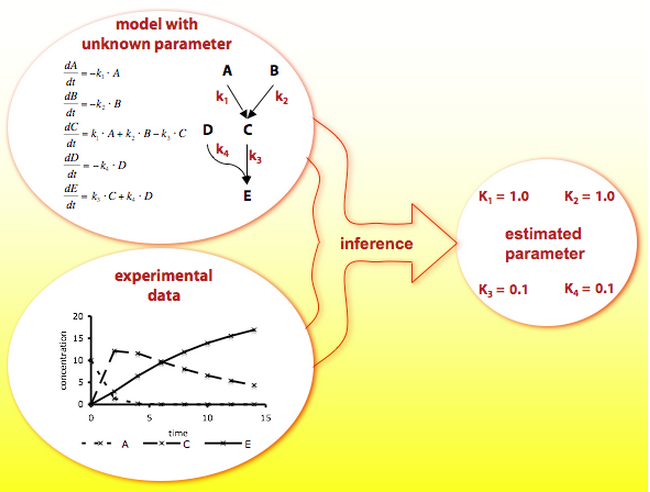
\includegraphics{../../fig/abcsysbio1.png}
\end{frame}

\begin{frame}
\frametitle{ABC-SysBio: a PyCUDA-implemented toolkit} \scriptsize
\setkeys{Gin}{width=1\textwidth} 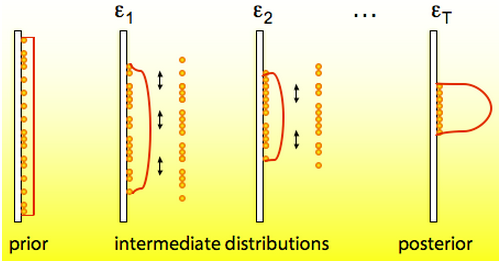
\includegraphics{../../fig/abcsysbio2.png}
\begin{itemize}
\item Methods
\begin{itemize}
\item ABC rejection sampler
\pause \item ABC SMC for parameter inference 
\pause \item ABC SMC for model selection
\end{itemize}
\end{itemize}
\end{frame}

\begin{frame}[fragile]
\frametitle{ABC-SysBio: a PyCUDA-implemented toolkit}
\begin{itemize}
\item ABC-SysBio is ready to use on impact1.
\begin{itemize}
\pause \item {\tt import abcsysbio} (Python script)
\pause \item {\tt  abc-sysbio-sbml-sum} (command line)
\pause \item {\tt run-abc-sysbio} (command line)
\end{itemize}
\pause \item For more information, visit:
\begin{itemize}
\item {\scriptsize \url{http://www.theosysbio.bio.ic.ac.uk/resources/abc-sysbio}}
\item {\scriptsize \url{http://bioinformatics.oxfordjournals.org/content/26/14/1797.full?keytype=ref\&ijkey=AVSfAhR7XFxjrMj}}
\end{itemize}
\pause \item For the input files in the online examples, visit:
\begin{itemize}
\item {\scriptsize \url{http://will-landau.com/gpu/pycuda.html}}
\end{itemize}
\end{itemize}
\end{frame}

\begin{frame}
\frametitle{Outline}
\tableofcontents
\end{frame}

\begin{frame}
\frametitle{Other resources}

\begin{itemize}
\item Guides and papers
\begin{itemize} \scriptsize 
\pause \item Klockner A. Examples of PyCUDA usage. \url{http://wiki.tiker.net/PyCuda/Examples}. May 2012.
\pause \item Klockner A. PyCUDA 2012.1 documentation. \url{http://documen.tician.de/pycuda/index.html}. June 2012.
\pause \item C. Barnes, J. Liepe, E. Cule, S. Filippi, D. Rolando, S. McMahon, B. Lisowska, P. Kirk, K. Erguler, T. Toni, and M. Stumpf. \emph{Abc-sysbio: A tool for parameter inference and model selection.} \url{http://www.theosysbio.bio.ic.ac.uk/resources/abc-sysbio}. 2011.
\pause \item J. Liepe, C. Barnes, E. Cule, K. Erguler, P. Kirk, T. Toni, and M. Stumpf. \emph{Abc-sysbio-approximate bayesian computation in Python with gpu support.} Bioinformatics, 26(14):1797�1799, May 2010.
\end{itemize}
\pause \item Example PyCUDA and ABC-SysBio code are available at \url{http://will-landau.com/gpu/pycuda.html}.
\end{itemize}
\end{frame}

\begin{frame}
\frametitle{That's all for the semester.}
\begin{itemize}
\item Series materials are available at \url{http://will-landau.com/gpu}.
\end{itemize}
\end{frame}

\end{document}